\section{Notes about GROMCACS usage}
\begin{figure}[htbp]
    \centering
    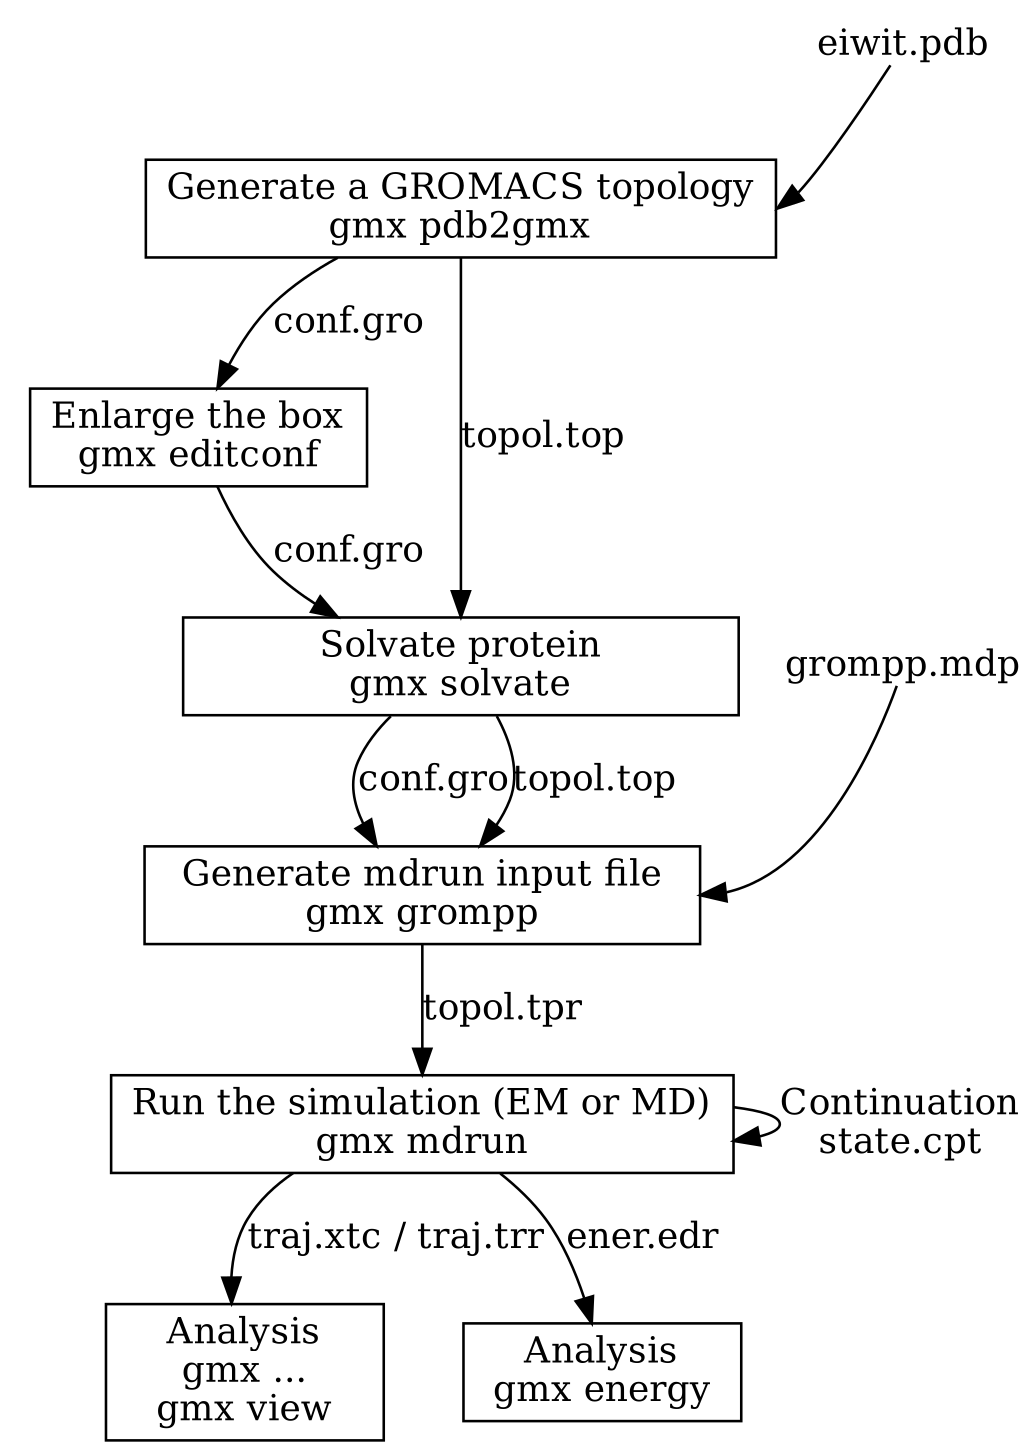
\includegraphics[width=.80\linewidth]{figures/flow-chart.png}
    \caption{Flow chart of GROMACS}
\end{figure}
Regarder comment faire un g(r) sur gromacs

\section{Deliverables}
Hydrate phase : $1 \times 2 \times 2$ unit cell with all its cavities filled with methane (184 water and 44 methane)\\
Methane gas phase: 160 methane molecules\\\\
1st liquid slab: 736 water molecules (pure liquid water slab)\\
2nd liquid slab: 736 water molecules and 128 methane molecules (liquid water slab supersaturated with methane)

Methane en united atoms, simulation plus simples, comparaison des résultats avec le papier de Tung

Bonded interactions on gromacs
Stretching ct hc
Bending hc ct hc

$kg.mol^-1.Angstroem^2 -> kJ.mol^-1.Angstroem^2$

SE RENSEIGNER SUR L'ANNEALING DANS GROMACS

Essayer de lancer les simul et de bidouiller jusqu'à ce que ça marche, puis me familiariser avec la commande gmx energy (xmgrace), une fois que ça marche, commencer à regarder thermostats/barostats/intégrateurs
Être en mesure de lancer les simulations NPT
Jeudi prochain -> parler de comment analyser les résultat
Analyse la plus importante -> caractérisation strucuturelle du système

Faire une première étape en berendsen
Une fois le volume stable, passer sur le barostat qui permet d'avoir un bon ensemble thermo

Une fois minimisé, première étape d'équilibration -> correspond à enlever la partie pression dans le coupling du groupe, changer la température, régler le nombre de steps pour avoir le bon temps (unité du pas de temps picoseconde)
Simulation sur 20 picosecondes

Pour les bonds, une fois minimisé -> remplacer none par h-bonds

ANALYSE

3 choses à coder :
paramètre d'ordre angulaire (aop)
g(r) (histogramme des distances)
détermination des liaisons hydrogène entre les molécules d'eau